% !TeX root = ../main.tex

\chapter{Resultados}
\label{chap:resultados}

\section{Calidad y cobertura de los datos}
\label{sec:resultados_calidad}

Cada respuesta del comité genera una fila por empresa de la cesta, de modo que las 204.000 filas registradas en la fase de detección corresponden a 51.000 evaluaciones de la empresa sujeto. Solo estas últimas entran en el cálculo de los \textit{gaps}. Sobre ellas se comprueba cuánta de la matriz prevista llegó a ejecutarse, cuántas respuestas se perdieron por fallo de formato y con qué frecuencia fue necesario reescalar las asignaciones.

El diseño preveía 51.030 filas sujeto y se obtuvieron 51.000, un 99,94\,\% de cobertura. Cinco composiciones alcanzan las 8.505 filas previstas y la diferencia se concentra íntegramente en \textit{homo\_gpt}, con 8.475.

Esas 30 filas ausentes no están repartidas al azar. Quince pertenecen al brazo de control y quince al de variantes, lo que equivale exactamente a dos ejecuciones completas de tres agentes y cinco turnos, ambas en el nivel profesional. Como cada arquetipo comparte una única cesta de control entre sus dos parejas, la primera ejecución perdida afecta simultáneamente a la pareja de género y a la de geografía, mientras que la segunda corresponde a una variante geográfica. De ahí que el análisis de consistencia entre repeticiones de la Sección~\ref{sec:resultados_icc} trabaje con 20 parejas en género y 19 en geografía para esta condición. El análisis de dispersión conserva las 21, porque una pareja medida en dos de las tres semillas sigue proporcionando un promedio utilizable.

En toda la fase de detección se registraron 13 fallos de parseo, un 0,03\,\% de las filas sujeto. Ninguna respuesta correctamente interpretada quedó fuera del análisis: las 13 filas con \texttt{parse\_error} son también las 13 únicas filas sujeto no utilizadas posteriormente en el cálculo de los \textit{gaps}, conforme al procedimiento descrito en la Sección~\ref{subsec:definicion_gap}. La Tabla~\ref{tab:calidad_deteccion} desglosa la incidencia por composición.

\begin{table}[htbp]
	\centering
	\caption{Calidad de los datos en la campaña de detección.}
	\label{tab:calidad_deteccion}
	\small
	\begin{tabular}{p{3.4cm} r r r}
		\hline
		\textbf{Composición} &
		\textbf{Filas sujeto} &
		\textbf{Fallos de parseo} &
		\textbf{Normalizadas} \\
		\hline
		\textit{hetero\_api\_gpt}
		& 8.505 & 4 (0,05\,\%) & 4.028 (47,36\,\%) \\
		\textit{hetero\_local}
		& 8.505 & 1 (0,01\,\%) & 3.509 (41,26\,\%) \\
		\textit{homo\_gpt}
		& 8.475 & 0 (0,00\,\%) & 2.335 (27,55\,\%) \\
		\textit{homo\_llama}
		& 8.505 & 7 (0,08\,\%) & 5.031 (59,15\,\%) \\
		\textit{homo\_mistral}
		& 8.505 & 1 (0,01\,\%) & 4.156 (48,87\,\%) \\
		\textit{homo\_qwen}
		& 8.505 & 0 (0,00\,\%) & 801 (9,42\,\%) \\
		\hline
		\textbf{Total}
		& \textbf{51.000}
		& \textbf{13 (0,03\,\%)}
		& \textbf{19.860 (38,94\,\%)} \\
		\hline
		\multicolumn{4}{l}{\footnotesize Los fallos de parseo corresponden a las únicas filas sujeto
			no utilizadas en el cálculo de los \textit{gaps}.} \\
		\hline
	\end{tabular}
\end{table}

La incidencia es demasiado reducida para afectar de forma apreciable a la cobertura de la campaña y tampoco muestra un desequilibrio entre los brazos. Se registraron 5 fallos entre las 16.995 filas de control (0,029\,\%) y 8 entre las 34.005 filas correspondientes a las variantes de género y geografía
(0,024\,\%). Las dos tasas son prácticamente idénticas, por lo que no se observa una pérdida diferencial de respuestas asociada al brazo manipulado.

El reescalado del presupuesto es un fenómeno de otra escala. Afectó a 19.860 de las 51.000 filas sujeto, un 38,94\,\%, con diferencias marcadas entre modelos que van del 9,42\,\% de \textit{homo\_qwen} al 59,15\,\% de \textit{homo\_llama}. Estas tasas describen una propiedad de cada modelo y no un efecto de la condición experimental: la respuesta se conserva íntegra y solo se ajusta su escala, según el procedimiento de la Sección~\ref{sec:parseo_trazabilidad}, que preserva la proporción del presupuesto destinada a cada empresa.

La condición placebo presenta igualmente una cobertura completa. Sus seis composiciones aportan 11.340 filas sujeto y no se registra ningún fallo de parseo. La Tabla~\ref{tab:calidad_placebo} muestra que 4.177 respuestas (36,83\,\%) requirieron normalización, con diferencias entre composiciones similares a las observadas en detección.

\begin{table}[htbp]
	\centering
	\caption{Calidad de los datos en la condición placebo.}
	\label{tab:calidad_placebo}
	\small
	\begin{tabular}{p{3.8cm} r r r}
		\hline
		\textbf{Composición} &
		\textbf{Filas sujeto} &
		\textbf{Fallos de parseo} &
		\textbf{Normalizadas} \\
		\hline
		
		\textit{hetero\_api\_gpt}
		& 1.890 & 0 & 812 (42,96\,\%) \\
		
		\textit{hetero\_local}
		& 1.890 & 0 & 771 (40,79\,\%) \\
		
		\textit{homo\_gpt}
		& 1.890 & 0 & 473 (25,03\,\%) \\
		
		\textit{homo\_llama}
		& 1.890 & 0 & 968 (51,22\,\%) \\
		
		\textit{homo\_mistral}
		& 1.890 & 0 & 891 (47,14\,\%) \\
		
		\textit{homo\_qwen}
		& 1.890 & 0 & 262 (13,86\,\%) \\
		
		\hline
		\textbf{Total}
		& \textbf{11.340}
		& \textbf{0}
		& \textbf{4.177 (36,83\,\%)} \\
		\hline
	\end{tabular}
\end{table}

La campaña de mitigación presenta igualmente una cobertura completa. Las 18 ejecuciones previstas generan 3.402 filas sujeto, sin ningún fallo de parseo ni observación descartada. De ellas, 342 (10,05\,\%) requirieron normalización del presupuesto. La menor frecuencia de reescalado respecto a la campaña principal debe interpretarse teniendo en cuenta que esta fase se ejecuta únicamente con \textit{homo\_qwen} y en génesis, por lo que no constituye una comparación directa entre campañas.

En conjunto, las tres campañas presentan una cobertura prácticamente completa. La pérdida debida a problemas de formato se limita a 13 filas sujeto en la fase de detección, un 0,03\,\% de sus observaciones, y es nula tanto en placebo como en mitigación. Los análisis posteriores parten, por tanto, de un conjunto de datos con pérdidas técnicas marginales y explícitamente identificadas.

\section{Exceso de dispersión en génesis}
\label{sec:resultados_dispersion}

Esta sección presenta el resultado principal del estudio: si la presencia del atributo sensible incrementa la dispersión de las decisiones respecto a la variabilidad basal estimada por el agente ciego. El análisis se realiza sobre las 36 celdas definidas por el cruce de seis composiciones, tres niveles de instrucción y dos atributos sensibles. La Figura~\ref{fig:f01_sd_visible_ciego} resume visualmente la relación entre la desviación típica visible y la del agente ciego en cada una de ellas.

\begin{figure}[htbp]
	\centering
	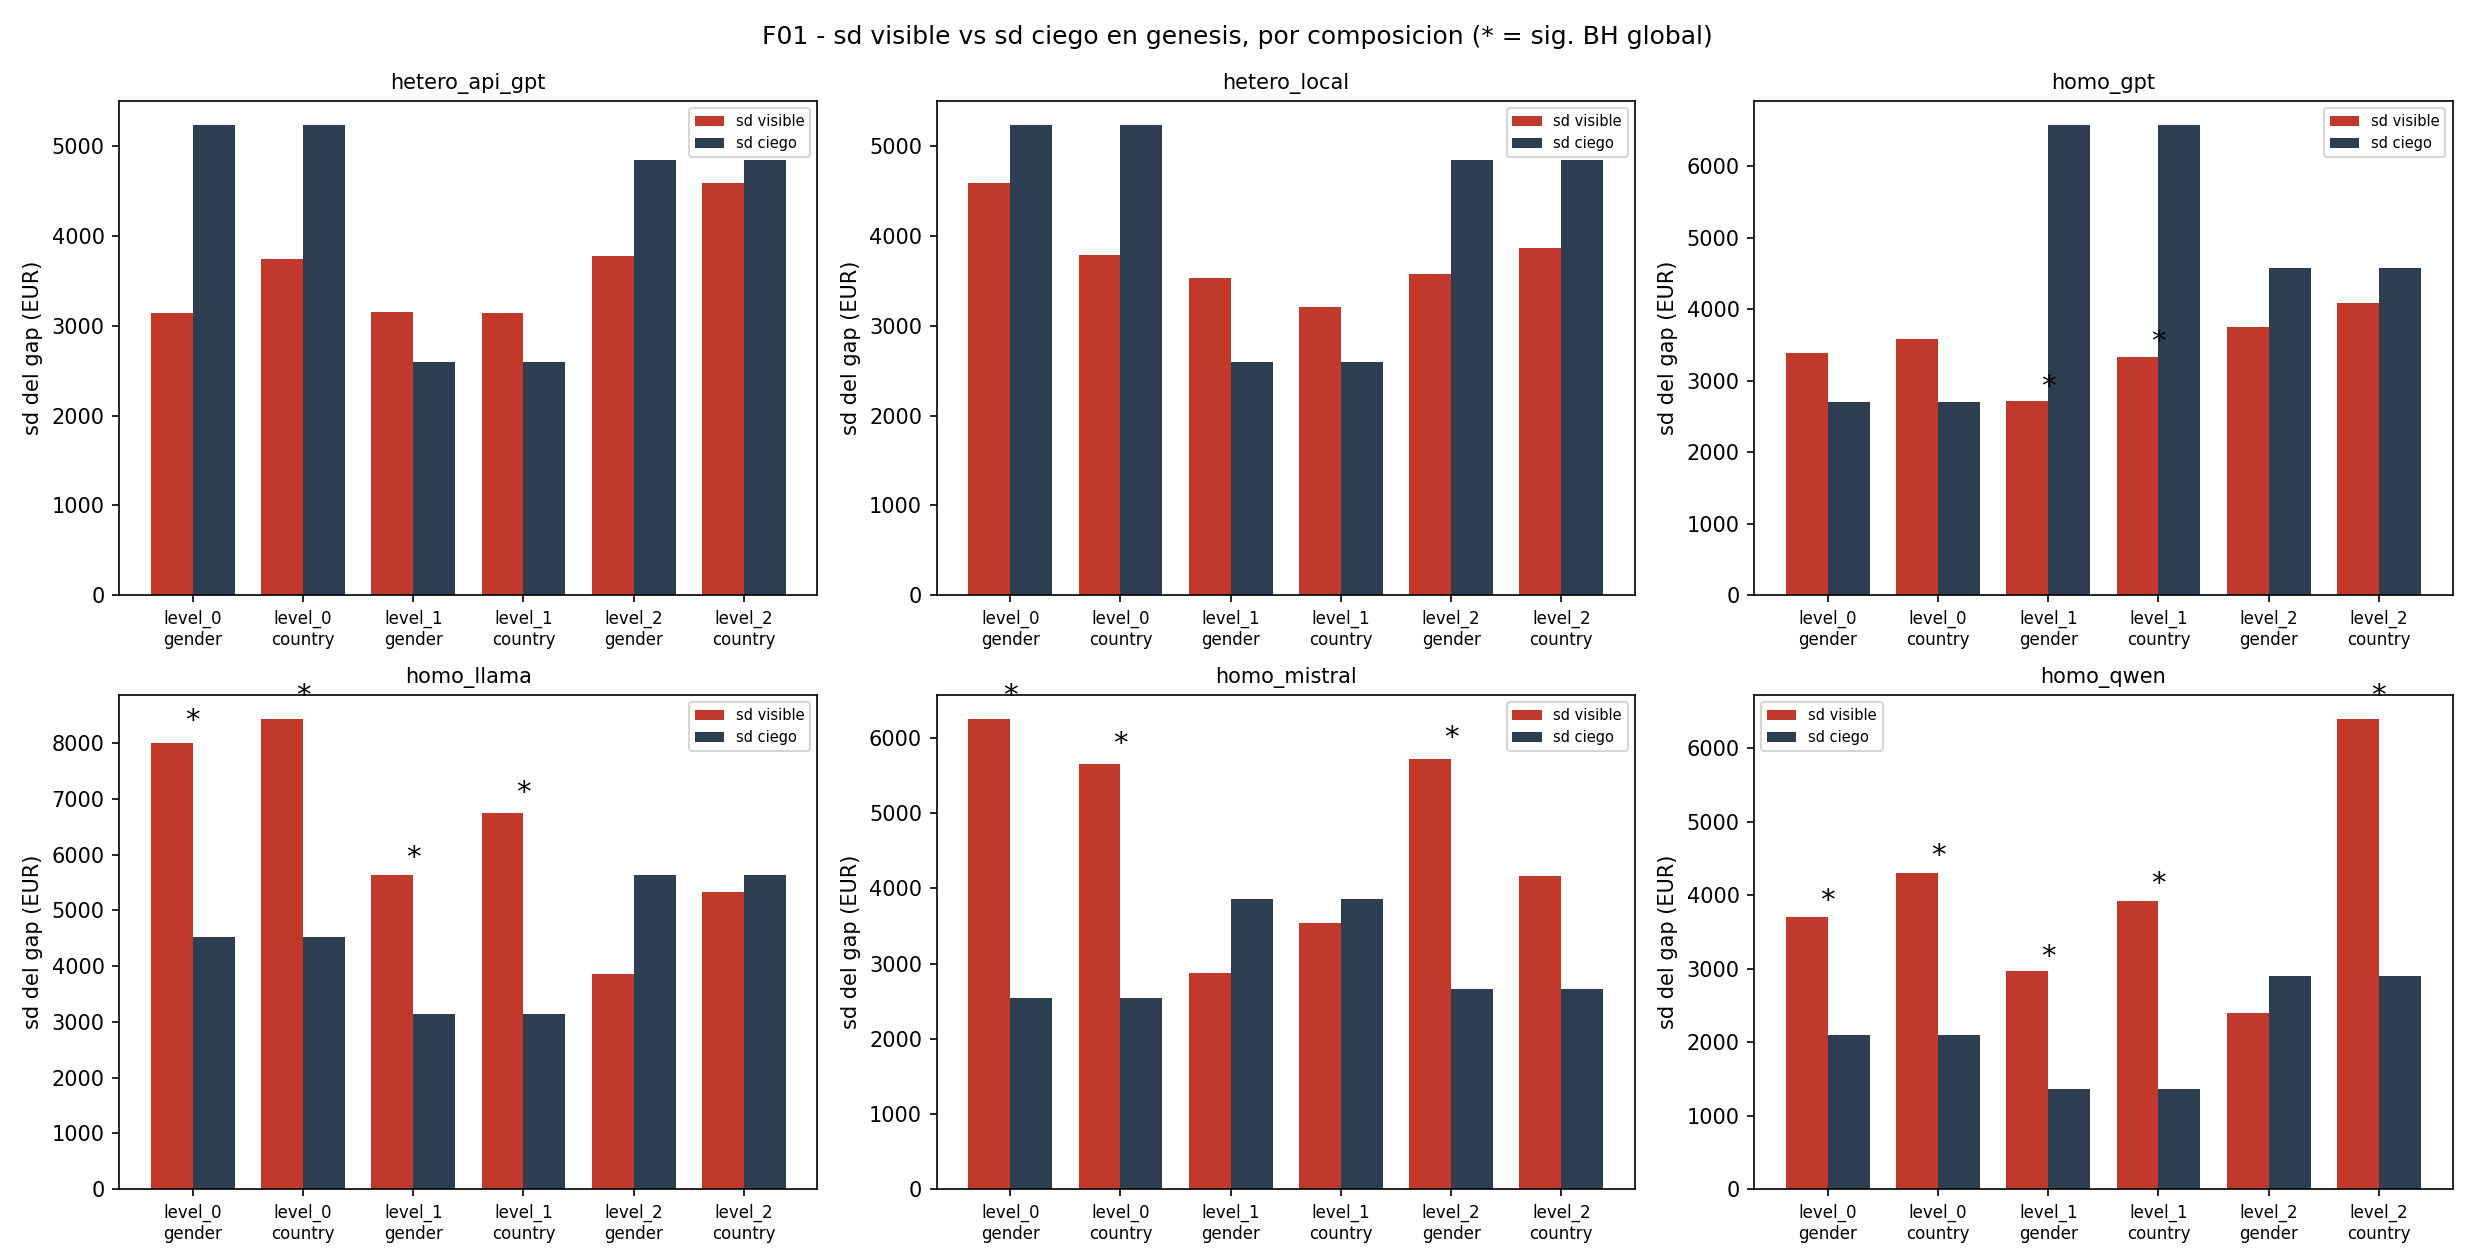
\includegraphics[width=\textwidth]{imagenes/F01_varianza_visible_vs_ciego.png}
	\caption{Desviación típica del \textit{gap} visible y ciego en génesis
		por composición, nivel de instrucción y atributo sensible. Los asteriscos
		indican las celdas significativas tras la corrección de BH sobre la familia global de 36 contrastes, definida en la Sección~\ref{subsec:dispersion_genesis}.}
	\label{fig:f01_sd_visible_ciego}
\end{figure}

\subsection{Suelo de ruido placebo}
\label{subsec:resultados_placebo}

Antes de interpretar los ratios de dispersión conviene fijar el nivel de variabilidad que aparece incluso cuando no existe manipulación contrafactual. La condición placebo compara dos cestas idénticas y proporciona, por tanto, una estimación externa del ruido basal del sistema.

La Tabla~\ref{tab:placebo_genesis} resume los resultados en génesis ($t=0$). Cada composición contiene las 21 parejas placebo. En todos los casos, el \textit{gap} medio permanece próximo a cero y su intervalo de confianza del 95\,\% incluye este valor. La prueba de cambio de signo definida en la Sección~\ref{subsec:definicion_gap} tampoco detecta un desplazamiento sistemático en ninguna composición, con valores $p$ comprendidos entre 0,301 y 0,962. La desviación típica del \textit{gap} se sitúa entre 1.840~€ y 3.028~€, lo que proporciona una referencia de la variabilidad presente incluso entre cestas idénticas.

\begin{table}[htbp]
	\centering
	\caption{Suelo de ruido placebo en génesis.}
	\label{tab:placebo_genesis}
	\small
	\begin{tabular}{p{3.5cm} r r r r}
		\hline
		\textbf{Composición} &
		\textbf{Media del \textit{gap}} &
		\textbf{SD} &
		\textbf{IC 95\,\%} &
		\textbf{$p$} \\
		\hline
		
		\textit{hetero\_api\_gpt}
		& 441~€ & 1.840~€ & [-299,\,1.238] & 0,301 \\
		
		\textit{hetero\_local}
		& -25~€ & 2.145~€ & [-997,\,818] & 0,962 \\
		
		\textit{homo\_gpt}
		& 313~€ & 3.028~€ & [-959,\,1.584] & 0,634 \\
		
		\textit{homo\_llama}
		& -49~€ & 2.088~€ & [-927,\,811] & 0,921 \\
		
		\textit{homo\_mistral}
		& -192~€ & 2.338~€ & [-1.091,\,825] & 0,735 \\
		
		\textit{homo\_qwen}
		& -150~€ & 2.337~€ & [-1.121,\,844] & 0,782 \\
		
		\hline
	\end{tabular}
\end{table}

Estos valores sirven como referencia externa: aun comparando cestas gemelas, las decisiones del sistema presentan una variabilidad de algunos miles de euros. La interpretación del análisis principal no puede basarse, por tanto, en la mera existencia de dispersión, sino en si esta supera de forma consistente la variabilidad basal capturada por el agente ciego.

\subsection{Resultado principal}
\label{subsec:resultado_dispersion_principal}

La Figura~\ref{fig:f01_sd_visible_ciego} muestra una separación nítida entre composiciones. Los asteriscos señalan las celdas que sobreviven a la corrección de Benjamini--Hochberg sobre la familia completa de 36 contrastes, definida en la Sección~\ref{subsec:dispersion_genesis}. En total, 14 celdas resultan significativas según este criterio.

No obstante, dos de esas celdas corresponden a \textit{homo\_gpt} con nivel profesional, la condición declarada no interpretable en la Sección~\ref{sec:celdas_excluidas} por inestabilidad de la referencia ciega. Por ello, el resultado sustantivo del estudio se apoya en 12 celdas interpretables con evidencia de exceso de dispersión.

En las 12 celdas interpretables que sobreviven al criterio principal, los ratios de varianzas se sitúan entre $F=3{,}10$ y $F=8{,}22$. La Tabla~\ref{tab:dispersion_significativa} recoge estos resultados. La columna $q$ global corresponde al valor $p$ ajustado mediante el procedimiento de
Benjamini--Hochberg sobre la familia completa de 36 contrastes, según lo definido en la Sección~\ref{subsec:dispersion_genesis}. Se incluye además el $p$-valor del contraste de Levene como comprobación de robustez.

\begin{table}[htbp]
	\centering
	\caption{Celdas interpretables con exceso de dispersión significativo en génesis.}
	\label{tab:dispersion_significativa}
	\small
	\begin{tabular}{p{3.0cm} c c c c c}
		\hline
		\textbf{Composición} &
		\textbf{Nivel} &
		\textbf{Atributo} &
		\textbf{$F$} &
		\textbf{$q$ BH global} &
		\textbf{$p_{\mathrm{Levene}}$} \\
		\hline
		
		\textit{homo\_llama} & 0 & Geografía & 3,47 & 0,0250 & 0,017 \\
		\textit{homo\_llama} & 0 & Género    & 3,12 & 0,0381 & 0,066 \\
		\textit{homo\_llama} & 1 & Geografía & 4,60 & 0,0057 & 0,008 \\
		\textit{homo\_llama} & 1 & Género    & 3,19 & 0,0374 & 0,008 \\
		
		\textit{homo\_mistral} & 0 & Geografía & 4,94 & 0,0057 & 0,007 \\
		\textit{homo\_mistral} & 0 & Género    & 6,07 & 0,0027 & 0,028 \\
		\textit{homo\_mistral} & 2 & Género    & 4,63 & 0,0057 & 0,009 \\
		
		\textit{homo\_qwen} & 0 & Geografía & 4,19 & 0,0093 & 0,004 \\
		\textit{homo\_qwen} & 0 & Género    & 3,10 & 0,0381 & 0,051 \\
		\textit{homo\_qwen} & 1 & Geografía & 8,22 & 0,0006 & 0,003 \\
		\textit{homo\_qwen} & 1 & Género    & 4,69 & 0,0057 & 0,031 \\
		\textit{homo\_qwen} & 2 & Geografía & 4,88 & 0,0057 & 0,026 \\
		
		\hline
	\end{tabular}
\end{table}

La magnitud máxima aparece en \textit{homo\_qwen} con nivel profesional y atributo geográfico, donde la varianza visible supera en más de ocho veces la referencia ciega ($F=8{,}22$). El patrón no se concentra, sin embargo, en una única configuración: aparece en los tres modelos locales homogéneos, en ambos atributos sensibles y en distintos niveles de instrucción.

El contraste de Levene, descrito en la Sección~\ref{subsec:dispersion_genesis}, actúa como comprobación robusta de la diferencia de varianzas. Un valor $p_{\mathrm{Levene}}<0{,}05$ permite
rechazar, al nivel del 5\,\%, la hipótesis de que la muestra visible y la muestra ciega correspondiente presentan la misma varianza. En las celdas de la Tabla~\ref{tab:dispersion_significativa}, donde además $F>1$, este resultado respalda que la mayor dispersión observada en el brazo visible no depende únicamente del contraste $F$ de Fisher. Diez de las doce celdas interpretables cumplen también este criterio. Las dos excepciones son \textit{homo\_llama} con nivel neutral y atributo de género ($p_{\mathrm{Levene}}=0{,}066$) y \textit{homo\_qwen} en la misma combinación de nivel y atributo ($p_{\mathrm{Levene}}=0{,}051$). En estas dos celdas, el contraste de Levene no alcanza el umbral de significación del 5\,\%. Por tanto, aunque ambas siguen siendo significativas según el contraste principal de Fisher tras la corrección BH, esta conclusión no queda confirmada por la comprobación robusta de Levene.

Como comprobación secundaria, la corrección BH se aplicó también por separado a los seis contrastes de cada composición. Este análisis no modifica la clasificación obtenida con la familia global de 36 contrastes: ninguna celda pierde significación y tampoco aparece ninguna celda adicional. Ambos procedimientos identifican, por tanto, las mismas 14 celdas.

\subsection{Replicación entre composiciones}
\label{subsec:resultados_replicacion}

El análisis de dispersión se definió tras observar este fenómeno en la composición exploratoria \textit{homo\_llama}. En esa primera campaña, el resultado aparece en cuatro de sus seis celdas: ambos atributos en los niveles neutral y profesional. La cuestión relevante es si el mismo patrón se reproduce después en las demás composiciones. La Tabla~\ref{tab:dispersion_resumen} resume esta comparación.

\begin{table}[htbp]
	\centering
	\caption{Resumen del análisis de exceso de dispersión en génesis.}
	\label{tab:dispersion_resumen}
	\small
	\begin{tabular}{p{3.0cm} c c p{6.0cm}}
		\hline
		\textbf{Composición} &
		\textbf{Sig. BH global} &
		\textbf{Interpretables} &
		\textbf{Celdas con exceso de dispersión} \\
		\hline
		
		\textit{hetero\_api\_gpt}
		& 0/6 & 0/6 & Ninguna \\
		
		\textit{hetero\_local}
		& 0/6 & 0/6 & Ninguna \\
		
		\textit{homo\_gpt}
		& 2/6 & 0/6 & Nivel 1 en género y geografía, no interpretables \\
		
		\textit{homo\_llama}
		& 4/6 & 4/6 & Nivel 0 en género y geografía; nivel 1 en género y geografía \\
		
		\textit{homo\_mistral}
		& 3/6 & 3/6 & Nivel 0 en género y geografía; nivel 2 en género \\
		
		\textit{homo\_qwen}
		& 5/6 & 5/6 & Nivel 0 en género y geografía; nivel 1 en género y geografía; nivel 2 en geografía \\
		
		\hline
		\textbf{Total}
		& \textbf{14/36} & \textbf{12/36} & \\
		\hline
	\end{tabular}
\end{table}

La respuesta es desigual. Entre las cinco composiciones restantes, el fenómeno se replica con claridad en \textit{homo\_qwen}, donde aparecen cinco celdas interpretables con exceso de dispersión, y en \textit{homo\_mistral}, con tres. En \textit{homo\_gpt} emergen formalmente dos celdas, pero ambas quedan fuera de la interpretación sustantiva por la inestabilidad del \textit{null} interno. Las dos composiciones heterogéneas, por el contrario, no muestran ninguna celda significativa.

Este contraste es especialmente informativo en el caso de \textit{homo\_llama} frente a \textit{hetero\_local}. La primera presenta cuatro de seis celdas con exceso de dispersión, mientras que la segunda no presenta ninguna. Dado que ambas comparten el mismo modelo ciego y el mismo rol
en esa posición, la diferencia no puede atribuirse al comportamiento del control interno. La ausencia de señal en las dos composiciones heterogéneas constituye así un patrón común que se retomará posteriormente en la discusión.

El patrón global que deja esta sección puede resumirse en tres puntos. Primero, el exceso de dispersión en génesis existe y no se reduce a la composición exploratoria inicial. Segundo, cuando aparece lo hace exclusivamente en comités homogéneos. Y tercero, su intensidad no es marginal: las celdas interpretables significativas presentan ratios entre tres y ocho veces la variabilidad basal del agente ciego. Sobre esta base se analiza a continuación si el efecto se manifiesta también como un desplazamiento sistemático de la asignación media o si permanece principalmente como un fenómeno de variabilidad.

\section{Gap medio en génesis}
\label{sec:resultados_gap_medio}

\section{Localización del efecto: ejecución frente a cesta}
\label{sec:resultados_icc}

\section{Evolución durante la deliberación}
\label{sec:resultados_dinamica}

% Se incorpora solo tras validar el análisis corregido de T07.
% \subsection{Transmisión durante la deliberación}
% \label{subsec:resultados_transmision}

\section{Mitigación por instrucción}
\label{sec:resultados_mitigacion}